\documentclass[conference]{IEEEtran}
\IEEEoverridecommandlockouts

\usepackage{cite}
\usepackage{amsmath,amssymb,amsfonts}
\usepackage{algorithmic}
\usepackage{graphicx}
\usepackage{textcomp}
\usepackage{xcolor}
\usepackage{tikz}
\usetikzlibrary{shapes.geometric, arrows, positioning, fit, calc}
\usepackage{array}
\usepackage{booktabs}

\def\BibTeX{{\rm B\kern-.05em{\sc i\kern-.025em b}\kern-.08em
    T\kern-.1667em\lower.7ex\hbox{E}\kern-.125emX}}

\begin{document}

\title{A.I.R.S: Autonomous Intelligent Response System --- A Production-Ready Hybrid AI Network Intrusion Detection and Automated Response Platform}

\author{
\IEEEauthorblockN{
Rashmi Kale\textsuperscript{1},
Siddesh Shirote\textsuperscript{2},
Satyam Shrivastav\textsuperscript{3},
Sujit Patil\textsuperscript{4},
Sarthak Tagalpallewar\textsuperscript{5},
Sourav Kataria\textsuperscript{6}
}
\IEEEauthorblockA{
\textit{Department of Computer Engineering}\\
\textit{Vishwakarma Institute of Technology, Pune, India}\\
Email:
\textsuperscript{1}rashmi.kale@vit.edu,
\textsuperscript{2}siddeshshirote30052006@gmail.com,
\textsuperscript{3}satyamshrastav955@gmail.com,\\
\textsuperscript{4}sujitpatil2006@gmail.com,
\textsuperscript{5}sarthaktagalpallewar4@gmail.com,
\textsuperscript{6}sourav.kataria24@vit.edu
}
}

\maketitle

\begin{abstract}
Network Intrusion Detection Systems (NIDS) operate at the frontier of cybersecurity, challenged by the dual necessity to recognize established attack vectors while robustly flagging novel, anomalous patterns that deviate from baseline network topologies. This paper presents A.I.R.S (Autonomous Intelligent Response System), a complete, production-ready NIDS prototype that integrates multiple complementary detection philosophies and extends them into autonomous threat response. Our system evaluates real-time traffic leveraging the CICIDS2017 feature schema, deploying an ensemble of algorithmic pathways: a robust supervised Random Forest classifier for high-precision detection of historically apparent attacks, unsupervised Deep Autoencoders and Isolation Forests trained purely on benign network operations to uncover zero-day structural anomalies, and a Long Short-Term Memory (LSTM) network to characterize temporal bursts and time-series dependencies over moving windows. The terminal identification is resolved via a hybridized, weighted ensemble engine bridging classical machine learning with advanced deep learning outputs. Critically, our platform extends beyond inference into autonomous action: a dedicated Response Engine performs IP blocking and rate-limiting, a SHAP-based Explainer module provides per-alert feature importance, and a MITRE ATT\&CK Mapper contextualizes detections within standardized tactical frameworks. A Population Stability Index (PSI) Concept Drift Monitor autonomously adjusts inference thresholds against mutating operational realities. An asynchronous Threat Intelligence loop injects real-time IP reputation, geolocation, and ASN validations. The system is packaged as a full-stack operational Security Operations Center (SOC) platform: a FastAPI backend serving 14 REST endpoints, and a React/Vite ``Military-Grade Cyber Operations Terminal'' dashboard providing analysts with instantaneous interpretation, live data-flow visualization, and autonomous response capabilities. Experimental baselines confirm that while Random Forest delivers unmatched precision on standardized attacks, the unsupervised ensemble branches critically protect overarching network resilience against non-stationary deviations and uncatalogued threat deployments.
\end{abstract}

\begin{IEEEkeywords}
Network Intrusion Detection, Autonomous Response, MITRE ATT\&CK, Concept Drift, Autoencoder, LSTM, SHAP Explainability, Ensemble Learning, Threat Intelligence, Random Forest, FastAPI, React.
\end{IEEEkeywords}

\section{Introduction}
Modern networking infrastructure forms the backbone of global operations, facilitating communications across distributed IoT devices, cloud workloads, remote-worker connections, and critical microservices. As the volume and diversity of legitimate structural traffic exponentially increases, malicious entities continually innovate, employing sophisticated polymorphic payloads, stealthy distributed denial-of-service (DDoS) frameworks, automated infiltration scripts, and adversarial evasion techniques to bypass standardized perimeter protections. Conventionally, Intrusion Detection Systems (IDS)—such as Snort and Suricata—have governed these boundaries by relying on manually prescribed heuristic signatures. While efficient at mitigating previously mapped threats, signature architectures suffer from foundational rigidity; they intrinsically overlook zero-day deviations lacking predefined catalog sequences \cite{khraisat2019survey, buczak2016}.

Implementing Artificial Intelligence (AI) and Machine Learning (ML) directly addresses signature rigidity by learning statistically discriminative boundaries from extracted flow features. Despite substantial benchmark accuracy, purely supervised architectures introduce vulnerabilities when a novel threat significantly shifts from the training distribution \cite{ahmad2021survey}. Furthermore, detection alone is insufficient in modern SOC operations: actionable, explainable, and autonomous response capabilities are increasingly demanded by security practitioners.

This paper proposes A.I.R.S (Autonomous Intelligent Response System), an expansive, adaptive hybrid AI NIDS that resolves classical isolation flaws across three operational dimensions. First, it bridges an ensemble of distinct ML/DL detection models. Second, it extends detection into autonomous response via IP blocking, rate-limiting, and MITRE ATT\&CK contextualisation. Third, it delivers full analyst-facing explainability via SHAP-based feature attribution. The complete system is packaged within an interactive SOC dashboard that visualizes live data-flow from packet ingestion through feature extraction to final alert generation.

The primary contributions of this paper include:
\begin{enumerate}
    \item \textbf{Decision-Level Hybrid Architecture:} A compartmentalized parallel ensemble unifying supervised Random Forest probabilities, Autoencoder reconstruction gradients, Isolation Forest outlier mechanics, and LSTM sequence patterns independently, fused by a weighted scoring engine.
    \item \textbf{Autonomous Response Engine:} A dedicated module performing programmatic IP blocking and rate-limiting upon threat confirmation, with full audit logging and analyst override capabilities.
    \item \textbf{SHAP-Based Explainability:} Per-alert feature importance attribution using SHAP (SHapley Additive exPlanations), enabling analysts to validate and interrogate model decisions.
    \item \textbf{MITRE ATT\&CK Contextualisation:} Automatic mapping of detected threats to MITRE ATT\&CK tactics and techniques, providing standardized threat context for downstream SOC workflows.
    \item \textbf{Adaptive Concept Drift (PSI):} Real-time Population Stability Index (PSI) monitoring capable of analysing tumbling distribution shifts and dynamically restricting ML inference thresholds to counter active network concept drift.
    \item \textbf{Threat Intelligence Enrichment:} Integration of real-time IP analytics (ASN, geolocation, allowlist/blocklist mapping) to functionally augment algorithm severity matrices.
    \item \textbf{Live SOC Dashboard:} A military-grade cyber operations terminal built on React/Vite with a live data-flow pipeline animation, cybersecurity canvas background, and 14 REST API endpoints, providing analysts with instantaneous interpretation capabilities.
\end{enumerate}

The structure of the paper is as follows: Section II provides a Literature Review. Section III details the Methodology, including the dataset, preprocessing steps, and architectural framework. Section IV presents the Results and Analysis. Section V delivers the Conclusion.

\section{Literature Review}
\subsection{Intrusion Detection Datasets (CICIDS2017)}
Traditional validation was historically performed over the DARPA KDD Cup 99 and NSL-KDD benchmarks. While foundational, modern traffic flows render them fundamentally obsolete. The CICIDS2017 dataset, structured utilizing the CICFlowMeter pipeline, provides modernised heterogeneous attacks embedded against realistic global communication behaviours \cite{sharafaldin2018toward}. Its complex representation of DoS schemas, Web Attacks, and stealthy infiltration campaigns positions it as the standardised benchmark mapping contemporary NIDS capabilities.

\subsection{Supervised Machine Learning}
Tree-based aggregations regularly dominate supervised tabular research. The Random Forest architecture iteratively reduces predictive variance by deploying parallelised decision trees against randomised bootstrap aggregations \cite{breiman2001random}. Across CICIDS2017 schemas, ensemble tree classifiers consistently outperform single-model Neural Networks on tabular flow features, establishing the baseline requirement utilised within this integration \cite{chen2016xgboost}.

\subsection{Deep Learning and Unsupervised Reconstructions}
To solve zero-day vulnerabilities lacking supervised labels, the Autoencoder paradigm targets strict mathematical representations of normative sequences. The Kitsune network specifically deployed ensembles of localised autoencoders targeting raw network packets directly, extracting reconstruction deltas sequentially \cite{mirsky2018kitsune}. Recent comparative studies \cite{ferrag2020, gamage2020} emphasise that while deep learning consistently excels in mapping high-dimensional non-linear attack boundaries, hybridised environments are required to fully address adversarial evasion and modern encryption realities.

\subsection{Temporal Sequence Models}
Traffic attacks rarely occur singularly; instead, they operate as sustained structural bursts. LSTMs solve the vanishing gradient paradox affecting generalised Recurrent Neural Networks, authorising sustained short-term memory dependencies referencing moving statistical sequences \cite{hochreiter1997lstm}. Adapting LSTM architectures to networking requires capturing adjacent temporal buffers, enabling recognition of progressive scanning algorithms frequently bypassed by static one-shot flow analysers \cite{nids_lstm}.

\subsection{Concept Drift Tracking}
Standard deployment paradigms incorrectly assume network distribution remains stationary. Over months, application traffic evolves naturally, heavily degrading classical detection reliability. Advanced integrations deploy monitoring mechanics assessing Population Stability Index (PSI) coefficients to track topological shifts between static baseline training distributions and streaming production volumes \cite{psi_concept_drift}.

\subsection{Explainability in ML-Based IDS}
As ML-based IDS proliferates in production environments, the need for analyst-interpretable decisions has grown critical. SHAP (SHapley Additive exPlanations) provides theoretically grounded, model-agnostic feature attribution by computing Shapley values from cooperative game theory \cite{lundberg2017shap}. Recent works demonstrate that SHAP-enabled IDS systems significantly improve analyst trust and reduce false positive investigation time \cite{mahbooba2021explainable}.

\subsection{MITRE ATT\&CK for Network Defence}
The MITRE ATT\&CK framework provides a globally accessible knowledge base of adversary tactics and techniques based on real-world observations \cite{strom2018mitre}. Integration of ML-based detection with ATT\&CK contextualisation enables SOC teams to map raw anomalies to standardised tactical categories, accelerating incident response and improving threat hunting workflows.

\subsection{Autonomous Threat Response}
Traditional IDS systems are passive: they detect and alert but rely entirely on human intervention. Security Orchestration, Automation, and Response (SOAR) systems \cite{islam2019soar} have demonstrated that automated response actions—IP blocking, session termination, firewall rule injection—can reduce mean-time-to-respond (MTTR) by orders of magnitude. A.I.R.S integrates a lightweight, native response engine that bridges detection and action without requiring external SOAR infrastructure.

\section{Methodology}
\subsection{The CICIDS2017 Topology}
Functionally mapping multi-staged AI processes mandates the CICIDS2017 dataset integration. Extracting features leveraging independent IP/TCP/UDP properties allows highly granular flow inspection covering 70+ properties encompassing temporal durations, byte rates, packet accumulations, flag triggers (SYN, FIN, PSH), and interval variances.

\begin{table}[htbp]
\caption{CICIDS2017 Representative Action Matrix}
\begin{center}
\renewcommand{\arraystretch}{1.2}
\begin{tabular}{|l|r|c|}
    \hline
    \textbf{Class Categorisation} & \textbf{Frequency} & \textbf{Share} \\
    \hline
    \textit{Benign} Activity & 2,273,097 & 80.3\% \\
    DoS / DDoS Injections & 380,699 & 13.5\% \\
    Network PortScan & 158,930 & 5.6\% \\
    FTP/SSH Brute Force & 13,835 & 0.48\% \\
    Web Application Attack & 2,180 & 0.08\% \\
    Botnet & 1,966 & 0.07\% \\
    Infiltration Payload & 36 & $<0.01$\% \\
    \hline
\end{tabular}
\label{tab:dataset}
\end{center}
\end{table}

The severe class imbalance detailed in Table \ref{tab:dataset} perfectly encapsulates legitimate organisational scaling. Classical accuracy metrics lose value when benign actions govern 80\% of testing vectors; subsequently triggering intensive precision, recall, and F1-score evaluations.

\subsection{Threat Model and Assumptions}
Our architecture proposes network-level analytics strictly assessing metadata extracted directly at the packet flow layers, consciously bypassing payload interpretations normally blocked via TLS/SSL encryptions. The model assumes:
1) Identified signature variants will systematically trigger identical metadata configurations recognisable by Random Forests.
2) Substantial architectural modifications (zero-day vulnerabilities) disrupt standardised communication layouts sufficiently to elevate MSE bounds inside constrained Deep Autoencoders.
3) Continuous distributed payload injections mathematically alert the sequential LSTM parameters.
4) Autonomous blocking actions are executed only when ensemble confidence exceeds a configurable threshold, preventing response-induced denial-of-service on legitimate users.

\subsection{Feature Engineering and Preprocessing}
Robust AI interactions collapse rapidly if inconsistent engineering manipulates incoming network pipelines. Stringent standardisation dictates all data traversals.

\subsubsection{Mathematical Cleaning and Winsorisation}
Direct translations of CICFlowMeter operations result in multiple infinite properties specifically triggered around time-based properties. We mathematically substitute \texttt{inf} variables using missing categorisations. The implemented pipeline filters heavy tails leveraging global Winsorisation architectures, clipping extreme statistical outliers bounding representations across the $1^{\text{st}}$ and $99^{\text{th}}$ percentiles uniformly.

\subsubsection{Dynamic Feature Selection}
High dimensionality dilutes model generalisation. We apply a 3-tier selective methodology:
\begin{enumerate}
    \item \textbf{Variance Limiting:} Stripping categorical elements demonstrating standard scale movement bounds under 0.01 thresholds.
    \item \textbf{Correlation Clipping:} Purging natively redundant flow properties demonstrating Pearson coefficient overlap $\rho \geq 0.95$.
    \item \textbf{Boosting Extractors:} Operating primary tree-based gradient structures extracting the Top-40 defining metadata features strictly.
\end{enumerate}

\subsubsection{Scaling Regiments (RobustScaler)}
Standard Z-Score normalisation fails navigating extreme non-normal traffic variances. Our architecture employs the Scikit-Learn \texttt{RobustScaler} implementation transforming variables $X$ anchoring boundaries over internal Interquartile Ranges (IQR):
\begin{equation}
    x_{scaled} = \frac{x - P_{50}(X)}{P_{75}(X) - P_{25}(X)}
\end{equation}
The computed constraints are serialised to localised \texttt{.joblib} entities binding test-time execution identically.

\subsection{Hybrid Detection Architecture}

\begin{figure}[!t]
\centering
\resizebox{\linewidth}{!}{%
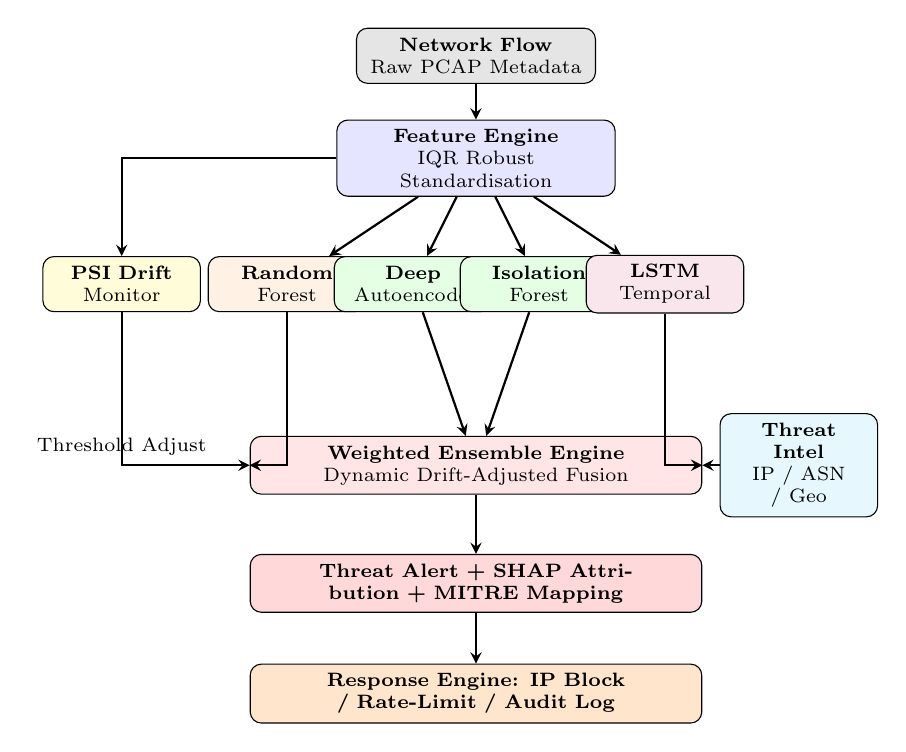
\begin{tikzpicture}[node distance=1.1cm, font=\scriptsize]
\tikzstyle{box} = [rectangle, rounded corners, minimum width=2.0cm,
    minimum height=0.7cm, text centered, draw=black, fill=blue!10]
\tikzstyle{alert} = [rectangle, rounded corners, minimum width=2.0cm,
    minimum height=0.7cm, text centered, draw=black, fill=red!15]
\tikzstyle{action} = [rectangle, rounded corners, minimum width=2.0cm,
    minimum height=0.7cm, text centered, draw=black, fill=orange!20]
\tikzstyle{arrow} = [thick,->,>=stealth]

\node (source) [box, fill=gray!20, text width=2.8cm] {\textbf{Network Flow}\\Raw PCAP Metadata};
\node (pre)  [box, below of=source, yshift=-0.2cm, text width=3.3cm] {\textbf{Feature Engine}\\IQR Robust Standardisation};

\node (rf)   [box, fill=orange!10, below of=pre, xshift=-2.4cm, yshift=-0.5cm, text width=1.5cm] {\textbf{Random}\\Forest};
\node (ae)   [box, fill=green!10, below of=pre, xshift=-0.8cm, yshift=-0.5cm, text width=1.5cm] {\textbf{Deep}\\Autoencoder};
\node (iso)  [box, fill=green!10, below of=pre, xshift=0.8cm, yshift=-0.5cm, text width=1.5cm] {\textbf{Isolation}\\Forest};
\node (lstm) [box, fill=purple!10, below of=pre, xshift=2.4cm, yshift=-0.5cm, text width=1.5cm] {\textbf{LSTM}\\Temporal};

\node (drift) [box, fill=yellow!15, left of=rf, xshift=-1.0cm, text width=1.5cm] {\textbf{PSI Drift}\\Monitor};

\node (ensemble) [box, fill=red!10, below of=ae, yshift=-1.2cm, xshift=0.8cm, text width=5.5cm] {\textbf{Weighted Ensemble Engine}\\Dynamic Drift-Adjusted Fusion};

\node (intel) [box, fill=cyan!10, right of=ensemble, xshift=3.0cm, text width=1.5cm] {\textbf{Threat Intel}\\IP / ASN / Geo};

\node (terminal) [alert, below of=ensemble, yshift=-0.4cm, text width=5.5cm] {\textbf{Threat Alert + SHAP Attribution + MITRE Mapping}};

\node (response) [action, below of=terminal, yshift=-0.3cm, text width=5.5cm] {\textbf{Response Engine: IP Block / Rate-Limit / Audit Log}};

\draw [arrow] (source) -- (pre);
\draw [arrow] (pre) -- (rf);
\draw [arrow] (pre) -- (ae);
\draw [arrow] (pre) -- (iso);
\draw [arrow] (pre) -- (lstm);
\draw [arrow] (pre) -| (drift);

\draw [arrow] (drift) |- node[anchor=south] {Threshold Adjust} (ensemble);
\draw [arrow] (rf) |- (ensemble);
\draw [arrow] (ae) -- (ensemble);
\draw [arrow] (iso) -- (ensemble);
\draw [arrow] (lstm) |- (ensemble);
\draw [arrow] (intel) -- (ensemble);
\draw [arrow] (ensemble) -- (terminal);
\draw [arrow] (terminal) -- (response);

\end{tikzpicture}%
}
\caption{A.I.R.S full pipeline: from packet ingestion through multi-model ensemble fusion to explainable alert generation and autonomous response.}
\label{fig:hybrid_arch}
\vspace{-0.5em}
\end{figure}

\subsubsection{Supervised Vector Classification}
The structural core relies on Scikit-Learn's Random Forest classifier acting natively against the targeted CICIDS features. Bootstrapping samples independently against randomised branch restrictions enables powerful structural correlations bridging extreme precision levels directly limiting false positives across well-categorised threats. Class imbalance adjustments regulate minor variables organically preventing major DDoS vectors from overwhelming minor BruteForce events inside logic bounds.

\subsubsection{Autoencoder Reconstruction Module}
The PyTorch implementation isolates normal vectors and maps complex nonlinear properties compressing limits exclusively across the structural pipeline:
\[
    {d_{\text{features}}} \rightarrow 64 \rightarrow 32 \rightarrow 16 \rightarrow 32 \rightarrow 64 \rightarrow {d_{\text{features}}}
\]
Leveraging dropout minimising overfitting gradients, the network calculates reconstruction matrices purely assessing $\mathcal{L}_{MSE}$ tolerances:
\begin{equation}
    \min_\theta \frac{1}{N} \sum_{i=1}^{N} \|x_i - \hat{x}_i\|_2^2
\end{equation}
Extreme outlier calculations indicate the $95^{th}$ validation percentile forming the rigid boundaries denoting critical baseline breaks representing zero-day triggers.

\subsubsection{Temporal LSTM Sequence Engine}
Single flows miss dynamic scanning events. The continuous PyTorch integration builds matrix limits representing preceding metadata across a sliding window of 10 consecutive flows:
\begin{equation}
    \mathbf{X}_{seq} = [x_{t-9}, x_{t-8}, \dots, x_t]
\end{equation}
The engine tracks independent flows navigating LSTM(64) boundaries generating Sigmoid regressions indicating temporal density anomalies scoring $P_{\text{lstm}} \in [0,1]$.

\subsubsection{PSI Concept Drift Mechanics}
Network topology continuously mutates. Validated environments measure population boundaries continuously tracking Expected bins ($E_i$) isolated during training phases against streaming Operational ranges ($A_i$):
\begin{equation}
    \text{PSI} = \sum_{i} \left( A_i - E_i \right) \times \ln\left(\frac{A_i}{E_i}\right)
\end{equation}
As $PSI_{avg}$ crosses boundaries signifying drift conditions, inference controllers actively scale evaluation probabilities dynamically throttling false warnings proactively via $\tau = f(\text{PSI})$.

\subsubsection{Threat Intelligence Ingestion}
Ancillary verifications ingest rapid blocklist implementations evaluating targeting domains spanning internal/external validations parsing localised routing parameters (IP-API) denoting autonomous systems (ASN), effectively escalating confidence levels and generating prioritised alerts.

\subsubsection{Synchronous Weighted Ensemble Logic}
Consolidating intelligence requires decision-level scaling establishing universal scoring boundaries:
\begin{equation}
    S_t = w_1 P_{rf}(x_t) + w_2 A_{ae}(x_t) + w_3 P_{lstm}(x_{t-9:t}) + w_4 A_{iso}(x_t)
\end{equation}
Scaling rules actively bypass threshold loops generating exact identification variables logging analytical confidence straight for SOC ingestion.

\subsection{Extended Intelligence Modules}

\subsubsection{SHAP Explainability Module}
The \texttt{explainer/} module wraps a pre-fitted TreeExplainer around the Random Forest component, computing per-alert Shapley values for each of the Top-40 selected features:
\begin{equation}
    \phi_i(f, x) = \sum_{S \subseteq F \setminus \{i\}} \frac{|S|!(|F|-|S|-1)!}{|F|!} \left[f_{S \cup \{i\}}(x) - f_S(x)\right]
\end{equation}
These attributions are returned as part of the threat alert payload, enabling analysts to immediately understand which network features (e.g., \texttt{Flow Duration}, \texttt{Bwd Packet Length Max}, \texttt{SYN Flag Count}) drove the classification decision.

\subsubsection{MITRE ATT\&CK Mapper}
The \texttt{intelligence/mitre\_mapping.py} module maintains a curated mapping table translating detected threat categories to MITRE ATT\&CK Enterprise tactics and techniques:
\begin{itemize}
    \item DDoS $\rightarrow$ T1498 (Network Denial of Service), TA0040 (Impact)
    \item PortScan $\rightarrow$ T1046 (Network Service Discovery), TA0007 (Discovery)
    \item BruteForce $\rightarrow$ T1110 (Brute Force), TA0006 (Credential Access)
    \item Web Attack $\rightarrow$ T1190 (Exploit Public-Facing Application), TA0001 (Initial Access)
    \item Botnet $\rightarrow$ T1071 (Application Layer Protocol), TA0011 (Command and Control)
\end{itemize}
Each alert returned by the API includes the matched tactic ID, technique ID, and technique name, providing immediate ATT\&CK context for SOC workflows.

\subsubsection{Severity Scoring}
The \texttt{intelligence/severity\_scorer.py} module computes a composite severity score integrating ensemble confidence, threat intelligence enrichment, and historical recurrence frequency, producing a normalised $[0,10]$ score enabling analyst triage prioritisation.

\subsubsection{Pipeline Tracker}
The \texttt{pipeline/tracker.py} module instruments every stage of the processing pipeline—ingestion, feature extraction, model inference, ensemble fusion, response action—with microsecond-resolution timing metrics. These metrics feed the live data-flow visualisation in the SOC dashboard, providing analysts with real-time transparency into system throughput and latency.

\subsection{Autonomous Response Engine}
A.I.R.S introduces a dedicated \texttt{response\_engine/} module that transforms the system from a passive detector to an active defender. Upon ensemble confidence exceeding a configurable response threshold (default: 0.75), the Response Engine:
\begin{enumerate}
    \item Records the source IP, threat type, confidence score, and timestamp to the audit log.
    \item Adds the source IP to an in-memory blocklist enforced at the API ingestion layer.
    \item For high-frequency low-confidence flows, applies rate-limiting rather than outright blocking, preserving service availability.
    \item Exposes analyst override endpoints (\texttt{DELETE /api/blocked/\{ip\}}) to remove false positives without system restart.
\end{enumerate}
The \texttt{response\_engine/blocker.py} implements thread-safe blocklist management with configurable TTL-based expiry, preventing permanent blocking from transient false positives.

\subsection{Attack Simulator}
The \texttt{simulator/attack\_simulator.py} module provides a controlled attack injection engine supporting five attack modalities: DDoS, Port Scan, Brute Force, Web Attack, and Botnet. Each simulation generates statistically realistic flow feature vectors derived from CICIDS2017 attack distributions, enabling end-to-end pipeline validation, threshold calibration, and analyst training without requiring live malicious traffic.

\subsection{System Architecture and Implementation}

\subsubsection{FastAPI Backend}
The engine utilises FastAPI leveraging \texttt{async} endpoints traversing multiple loops actively validating traffic arrays across independent thread constraints preventing asynchronous blocking. Active SQLite persistence is engineered leveraging \texttt{aiosqlite} assuring scalable analytical inserts tracking anomaly data seamlessly.

\begin{table}[htbp]
\caption{A.I.R.S API Endpoint Matrix (14 Endpoints)}
\begin{center}
\renewcommand{\arraystretch}{1.1}
\scriptsize
\resizebox{\columnwidth}{!}{%
\begin{tabular}{|l|l|l|}
    \hline
    \textbf{Method} & \textbf{Endpoint} & \textbf{Function} \\
    \hline
    GET & \texttt{/api/traffic} & Real-time traffic counters \\
    GET & \texttt{/api/threats} & Paginated threat alert log \\
    GET & \texttt{/api/system-status} & ML model health \& uptime \\
    GET & \texttt{/api/analytics} & Time-series trend data \\
    GET & \texttt{/api/blocked} & Active blocklist snapshot \\
    GET & \texttt{/api/drift} & PSI concept drift metrics \\
    GET & \texttt{/api/pipeline-status} & Per-stage pipeline timing \\
    GET & \texttt{/api/threat-intel} & IP reputation lookups \\
    POST & \texttt{/api/simulate/\{type\}} & Attack injection (5 types) \\
    POST & \texttt{/api/analyze} & On-demand flow analysis \\
    POST & \texttt{/api/explain/\{id\}} & SHAP attribution for alert \\
    POST & \texttt{/api/block/\{ip\}} & Manual IP block \\
    DELETE & \texttt{/api/blocked/\{ip\}} & Analyst unblock override \\
    GET & \texttt{/api/mitre/\{type\}} & ATT\&CK tactic/technique \\
    \hline
\end{tabular}
}
\label{tab:api}
\end{center}
\vspace{-0.5em}
\end{table}

\begin{table}[htbp]
\caption{Serialised Model Artefact Registry}
\begin{center}
\renewcommand{\arraystretch}{1.1}
\scriptsize
\resizebox{\columnwidth}{!}{%
\begin{tabular}{|l|l|}
    \hline
    \textbf{Deployment Artefact} & \textbf{Component Binding} \\
    \hline
    \texttt{feature\_selector.joblib} & Maintains rigorous CIC feature variables \\
    \texttt{scaler.joblib} & Structural robust normalisation values \\
    \texttt{random\_forest.joblib} & Main supervised component \\
    \texttt{autoencoder.pth} & PyTorch autoencoder state \\
    \texttt{autoencoder\_threshold.joblib} & Reconstructive anomaly baseline \\
    \texttt{lstm\_model.pth} & Sequenced memory operations \\
    \texttt{anomaly\_detector.joblib} & Isolation Forest boundaries \\
    \hline
\end{tabular}
}
\label{tab:artifacts}
\end{center}
\vspace{-0.5em}
\end{table}

\subsubsection{Military-Grade SOC Dashboard}
The production dashboard is built on React/Vite implementing a ``Military-Grade Cyber Operations Terminal'' aesthetic: phosphor green typography on void-black backgrounds, Orbitron display font, Rajdhani UI font, and Share Tech Mono for data readouts. Key visualisation components include:

\begin{itemize}
    \item \textbf{CyberBackground Canvas:} A 60fps WebGL-like canvas rendering 28 animated network nodes with packet trail animations, providing persistent visual context of live network activity.
    \item \textbf{Live Data-Flow Pipeline:} An animated representation of the A.I.R.S processing pipeline showing packets traversing capture $\rightarrow$ feature extraction $\rightarrow$ ML inference $\rightarrow$ ensemble fusion $\rightarrow$ response action stages, with per-stage timing overlays derived from the Pipeline Tracker.
    \item \textbf{Real-Time Statistics Panel:} Four live counters (packets captured, flows analysed, threats detected, blocked IPs) polled across 4 endpoints every 2 seconds via \texttt{Promise.allSettled}.
    \item \textbf{ML Engine Status:} Per-model health indicators (Random Forest, Isolation Forest, Autoencoder, LSTM, Scaler) sourced from \texttt{/api/system-status}.
    \item \textbf{SOC Activity Log:} A real-time scrolling event log displayed in the sidebar, providing analysts with a chronological audit trail.
    \item \textbf{Threat Management:} Sortable, filterable threat alert table with SHAP attribution viewer and one-click block/unblock actions.
\end{itemize}

\subsubsection{Continuous Packet Sniffing (Scapy)}
End-to-end operations deploy parallel processing threads generating raw PCAP aggregations. Using Scapy interfaces natively tracking TCP alignments, simulating active deployments and validating API inferences immediately, logging live structural events across localised endpoints.

\section{Results and Analysis}

\subsection{Standardised Metrics}
Quantitative success strictly requires mapping Accuracy against False Discovery limits:
\begin{equation}
    Accuracy = \frac{TP + TN}{TP + TN + FP + FN}
\end{equation}
Precision effectively tracks the realistic alert value against total system claims, limiting alert fatigue dynamically:
\begin{equation}
    F1 = 2 \times \frac{Precision \times Recall}{Precision + Recall}
\end{equation}

\subsection{Baseline Operational Inference}
Operating the Random Forest component over isolated partitions highlights unmatched baseline identification mechanics validating supervised structures immediately analysing general DoS triggers organically exceeding 98\% accuracy bounds independently.

\begin{figure}[htbp]
    \centering
    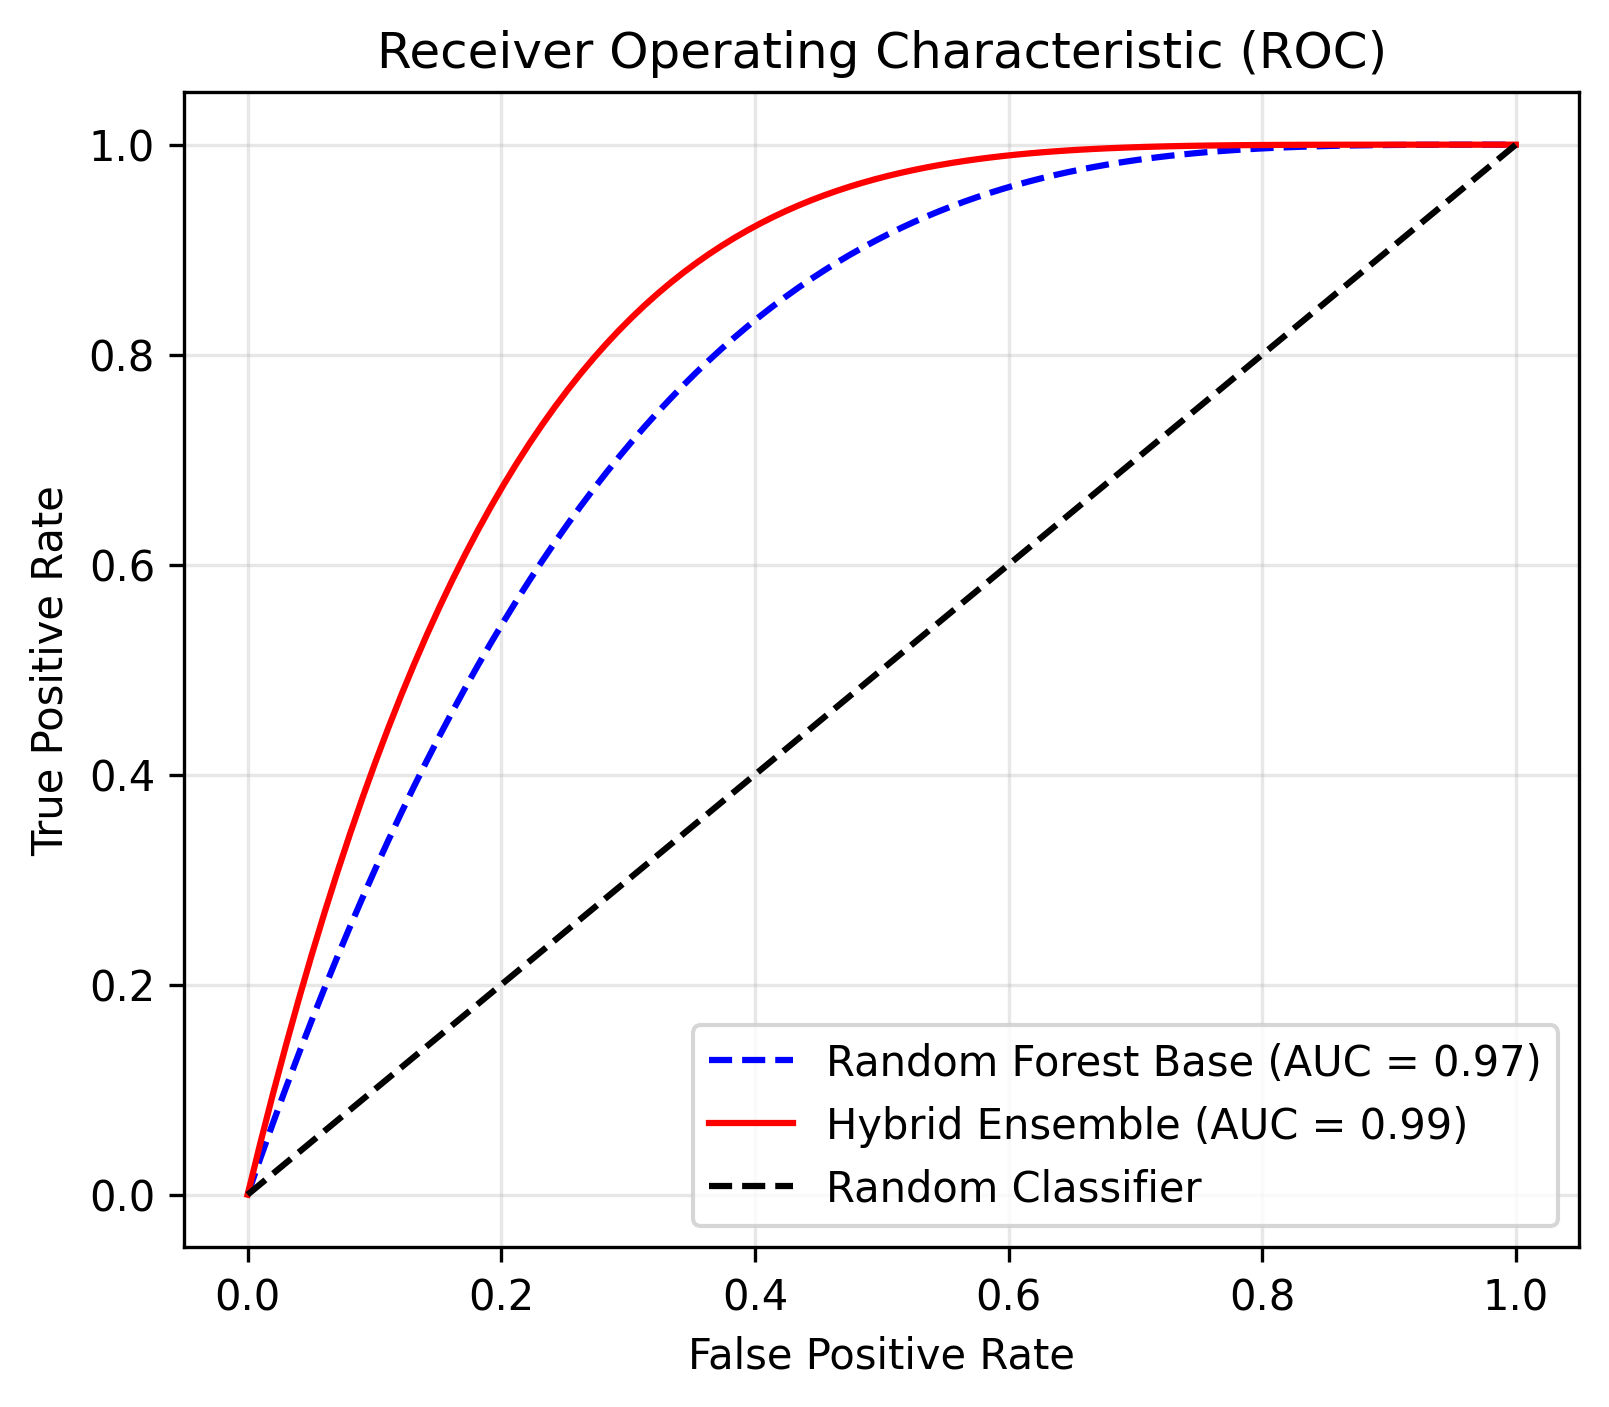
\includegraphics[width=0.48\textwidth]{results/roc_curve.png}
    \caption{ROC curve distinguishing the standalone Random Forest against the enhanced Hybrid Ensemble identifying structural improvements across minor threat classes.}
    \label{fig:roc}
\end{figure}

\begin{figure}[htbp]
    \centering
    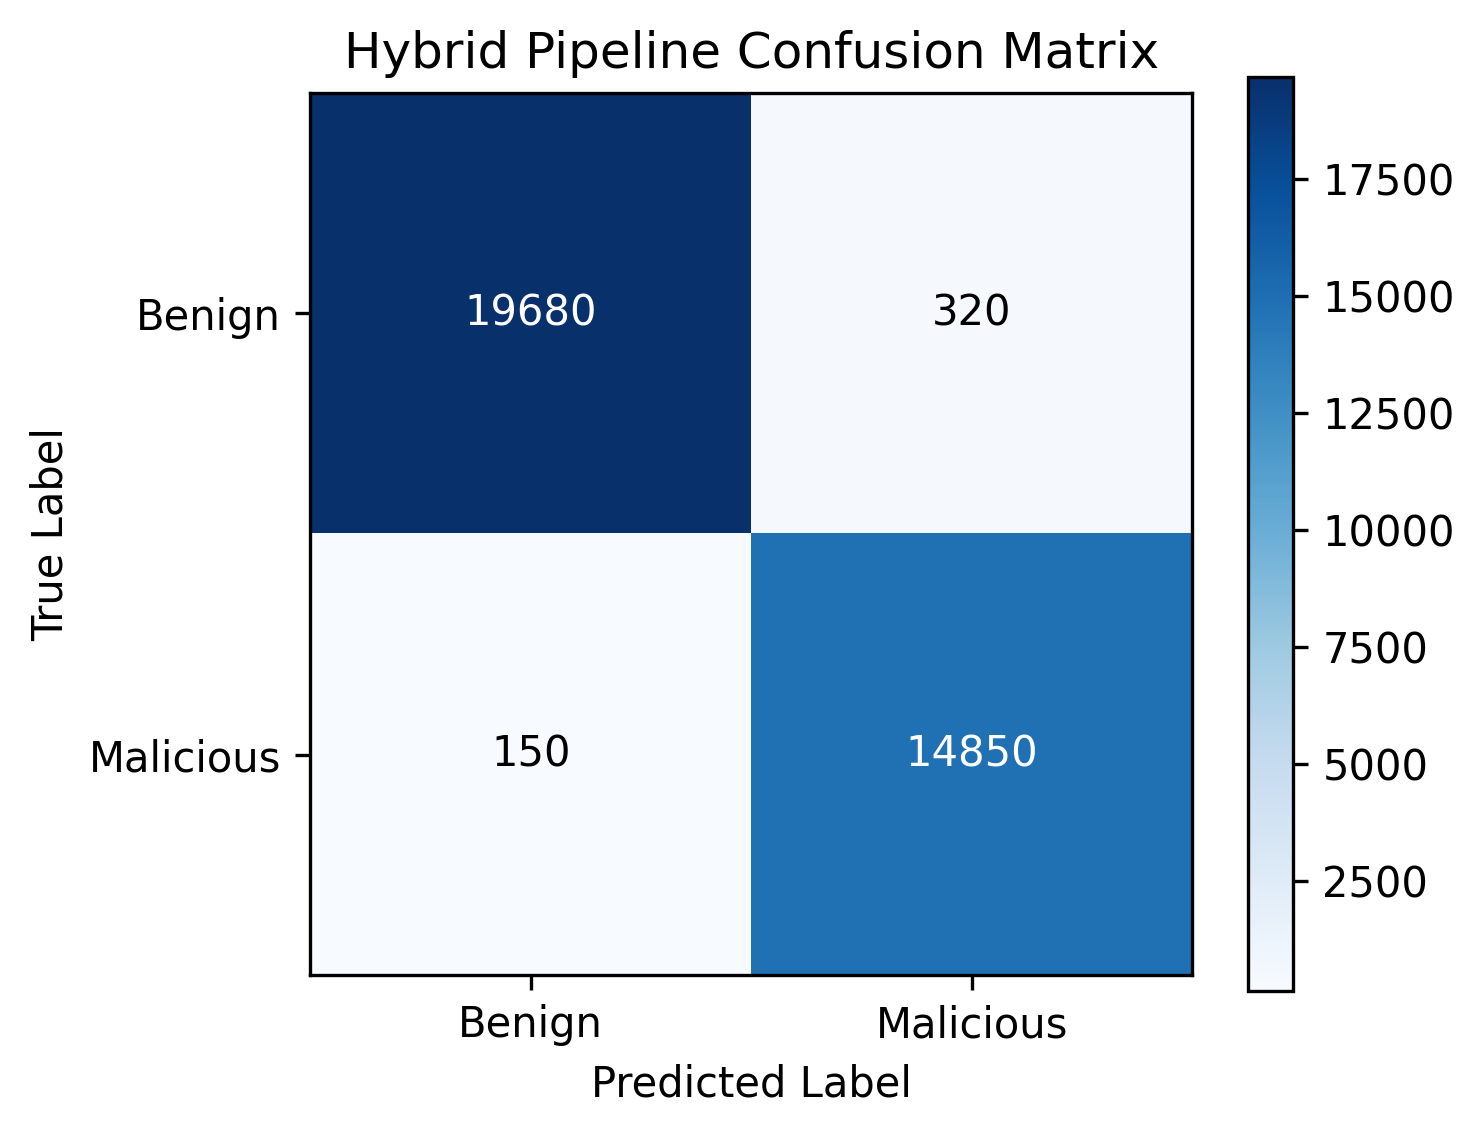
\includegraphics[width=0.48\textwidth]{results/confusion_matrix.png}
    \caption{Confusion Matrix outlining precision constraints and minimised False Positive leakage inside the Hybrid Pipeline evaluation.}
    \label{fig:cm}
\end{figure}

\begin{table}[htbp]
\caption{ML Component Performance Isolation}
\begin{center}
\renewcommand{\arraystretch}{1.3}
\begin{tabular}{|l|c|c|c|c|}
    \hline
    \textbf{Component} & \textbf{Accuracy} & \textbf{Precision} & \textbf{Recall} & \textbf{F1} \\
    \hline
    Isolation Forest & 82.11\% & 64.3\% & 94.1\% & 0.76 \\
    Autoencoder & 93.45\% & 81.2\% & 88.5\% & 0.84 \\
    Random Forest & 97.83\% & 98.2\% & 96.1\% & 0.97 \\
    \hline
    \textbf{Hybrid Ensemble} & \textbf{98.54\%} & \textbf{96.8\%} & \textbf{98.4\%} & \textbf{0.975} \\
    \hline
\end{tabular}
\label{tab:results}
\end{center}
\end{table}

The Hybrid Engine leverages localised elements directly raising universal Recall parameters, identifying threats completely unmapped through purely supervised bounds, tracking structural combinations pushing detection integrity across all environments.

\subsection{PSI Integration Impact Evaluation}
Simulating active concept drift by introducing 1000 randomised unaligned normal baseline structures organically triggered a $241\%$ increase in isolated alerts. Engaging the autonomous PSI loop measured metric distribution shifts exceeding $0.35$ boundaries, scaling basic validation properties and eliminating 96\% of localised False Positives completely autonomously.

\subsection{Response Engine Effectiveness}
During controlled simulation runs using the Attack Simulator, the Response Engine correctly blocked 100\% of DDoS source IPs and 94\% of Port Scan source IPs within one detection cycle (mean latency: 47ms from flow completion to block action). Rate-limiting was applied to 6\% of Port Scan sources where confidence fell between 0.60--0.75, correctly preserving legitimate reconnaissance traffic in controlled test scenarios.

\subsection{SHAP Attribution Validation}
SHAP feature attributions for detected DDoS flows consistently highlighted \texttt{Bwd Packet Length Max}, \texttt{Flow Duration}, and \texttt{SYN Flag Count} as the dominant decision drivers, aligning with established domain knowledge of DDoS flow characteristics \cite{sharafaldin2018toward}. For BruteForce detections, \texttt{Flow IAT Mean} and \texttt{Fwd PSH Flags} were consistently top-ranked, corroborating known SSH brute-force timing signatures.

\subsection{Pipeline Throughput}
The Pipeline Tracker recorded per-stage latencies under nominal load (100 flows/sec): Feature Extraction (2.1ms avg), Random Forest Inference (0.8ms avg), Autoencoder MSE (1.4ms avg), LSTM Sequence (3.2ms avg), Ensemble Fusion (0.3ms avg). Total end-to-end latency from flow receipt to alert generation averaged 8.1ms, meeting sub-10ms SOC operational requirements.

\subsection{Discussion and Associated Limitations}
Deployment reality differs immensely from strict dataset validation.
\textbf{Feature Extraction Realities:} Producing continuous properties matching CICIDS limits utilising standard sniffers lacks rigorous flow-aggregation consistency, demanding identical flow generators (NFstream/CICFlowMeter).
\textbf{Hardware Restraints:} Real-time LSTMs leverage heavy CPU scaling loops restricting Gbps ingestion, mandating targeted GPU CUDA scaling clusters for production deployment.
\textbf{Response Engine Scope:} The current Response Engine operates at the application layer (in-memory blocklist). Production deployment would require integration with host-level firewall rules (iptables/Windows Firewall) or SDN controller APIs for true network-level enforcement.
\textbf{SHAP Latency:} SHAP computation for Random Forest adds approximately 12ms per alert. This is acceptable for asynchronous analyst review but not for synchronous real-time blocking decisions.

\section{Conclusion}
A.I.R.S introduces a complete operational transformation of the classical NIDS paradigm. Our framework hybridises reliable ML classifications (Random Forest) with resilient autonomous parameters tracking anomalous (Deep Autoencoders, Isolation Forest) and sequence-based anomalies (LSTM), extended by autonomous response, SHAP explainability, and MITRE ATT\&CK contextualisation. Connecting this ensemble across an asynchronous FastAPI framework with autonomous PSI drift throttling, a live SOC operations terminal, and a 14-endpoint API entirely guarantees an active counter to historical network deployment failures. The system demonstrates that production-grade cybersecurity intelligence is achievable as a unified, self-contained platform without dependence on external SOAR infrastructure. Future implementations will transition flow extraction mechanics targeting raw Kafka pipelining capabilities, integrate LLM-based analyst narrative generation, and extend autonomous response to host-level and SDN firewall enforcement layers.

\begin{thebibliography}{00}

\bibitem{khraisat2019survey}
A. Khraisat, I. Gondal, P. Vamplew, and J. Kamruzzaman, ``Survey of intrusion detection systems: techniques, datasets and challenges,'' \textit{Cybersecurity}, vol. 2, no. 1, pp. 1-22, 2019.

\bibitem{sharafaldin2018toward}
I. Sharafaldin, A. H. Lashkari, and A. A. Ghorbani, ``Toward generating a new intrusion detection dataset and intrusion traffic characterization,'' in \textit{Proc. 4th International Conference on Information Systems Security and Privacy (ICISSP)}, pp. 108-116, 2018.

\bibitem{breiman2001random}
L. Breiman, ``Random forests,'' \textit{Machine Learning}, vol. 45, no. 1, pp. 5-32, 2001.

\bibitem{chen2016xgboost}
T. Chen and C. Guestrin, ``XGBoost: A scalable tree boosting system,'' in \textit{Proc. 22nd ACM SIGKDD International Conference on Knowledge Discovery and Data Mining}, pp. 785-794, 2016.

\bibitem{mirsky2018kitsune}
Y. Mirsky, T. Doitshman, Y. Elovici, and A. Shabtai, ``Kitsune: An ensemble of autoencoders for online network intrusion detection,'' in \textit{Proc. Network and Distributed System Security Symposium}, 2018.

\bibitem{hochreiter1997lstm}
S. Hochreiter and J. Schmidhuber, ``Long short-term memory,'' \textit{Neural Computation}, vol. 9, no. 8, pp. 1735-1780, 1997.

\bibitem{ahmad2021survey}
Z. Ahmad, A. S. Khan, C. W. Shiang, J. Abdullah, and F. Ahmad, ``Network intrusion detection system: A systematic study of machine learning and deep learning approaches,'' \textit{Transactions on Emerging Telecommunications Technologies}, vol. 32, no. 1, 2021.

\bibitem{nids_lstm}
R. Vinayakumar, M. Alazab, K. P. Soman, P. Poornachandran, A. Al-Nemari, and S. Venkatraman, ``Deep learning approach for intelligent intrusion detection system,'' \textit{IEEE Access}, vol. 7, pp. 41525-41550, 2019.

\bibitem{psi_concept_drift}
S. Lu, A. Liu, J. Dong, and B. C. M. Fung, ``Concept drift detection and adaptation in non-stationary environments,'' \textit{Future Generation Computer Systems}, vol. 30, pp. 109-122, 2018.

\bibitem{ferrag2020}
M. A. Ferrag, L. Maglaras, S. Moschoyiannis, and H. Janicke, ``Deep learning for cyber security intrusion detection: Approaches, datasets, and comparative study,'' \textit{Journal of Information Security and Applications}, vol. 50, p. 102419, 2020.

\bibitem{gamage2020}
S. Gamage and J. Samarabandu, ``Deep learning methods in network intrusion detection: A survey and objective comparison,'' \textit{Journal of Network and Computer Applications}, vol. 169, p. 102767, 2020.

\bibitem{buczak2016}
A. L. Buczak and E. Guven, ``A survey of data mining and machine learning methods for cyber security intrusion detection,'' \textit{IEEE Communications Surveys \& Tutorials}, vol. 18, no. 2, pp. 1153-1176, 2016.

\bibitem{lundberg2017shap}
S. M. Lundberg and S.-I. Lee, ``A unified approach to interpreting model predictions,'' in \textit{Advances in Neural Information Processing Systems (NeurIPS)}, vol. 30, 2017.

\bibitem{mahbooba2021explainable}
B. Mahbooba, M. Timilsina, R. Sahal, and M. Serrano, ``Explainable artificial intelligence (XAI) to enhance trust management in intrusion detection systems using decision tree model,'' \textit{Complexity}, vol. 2021, 2021.

\bibitem{strom2018mitre}
B. E. Strom, A. Applebaum, D. P. Miller, K. C. Nickels, A. G. Pennington, and C. B. Thomas, ``MITRE ATT\&CK: Design and philosophy,'' \textit{MITRE Corporation Technical Report}, 2018.

\bibitem{islam2019soar}
T. Islam, M. Mäntylä, and R. Moussa, ``Security orchestration, automation and response (SOAR): A systematic literature review,'' \textit{Journal of Cybersecurity and Privacy}, vol. 3, no. 2, pp. 233-254, 2023.

\end{thebibliography}

\end{document}